\documentclass[11pt]{article}

\usepackage{amsmath}
\usepackage{amssymb}
\usepackage[margin=0.68in]{geometry}
\usepackage{booktabs}
\usepackage{enumitem}
\usepackage{fancyhdr}
\usepackage{graphicx}
\usepackage[table]{xcolor}
\usepackage[hidelinks]{hyperref}
\usepackage{listings}
\usepackage{microtype}
\usepackage{tabularx}
\usepackage{tikz}
\usepackage{titlesec}
\usetikzlibrary{arrows.meta,positioning}
\graphicspath{{docs/lessons/assets/}{../assets/}}

\definecolor{AdkBlue}{gray}{0}
\definecolor{AdkRed}{gray}{0}
\definecolor{AdkGreen}{gray}{0.20}
\definecolor{CodeGray}{gray}{0.96}
\hypersetup
{
    pdftitle={ADK Lesson 011: Timed Traffic Controller},
    pdfauthor={Kevin Shanahan},
    pdfsubject={Deterministic nonblocking state transitions and pedestrian requests},
    pdflang={en-US}
}
\pagestyle{fancy}
\fancyhf{}
\lhead{\textsc{ADK Lesson 011}}
\rhead{Timed Traffic Controller}
\cfoot{\thepage}
\setlength{\headheight}{14pt}
\setlength{\parindent}{0pt}
\setlength{\parskip}{5pt}
\setlist{nosep,leftmargin=1.45em}
\titleformat{\section}{\Large\bfseries\color{AdkBlue}}{\thesection}{0.5em}{}
\titleformat{\subsection}{\large\bfseries\color{AdkBlue}}{\thesubsection}{0.5em}{}
\lstdefinestyle{adkcpp}
{
    language=C++,
    backgroundcolor=\color{CodeGray},
    basicstyle=\ttfamily\small,
    keywordstyle=\color{AdkBlue}\bfseries,
    commentstyle=\color{AdkGreen},
    columns=fullflexible,
    keepspaces=true,
    showstringspaces=false,
    frame=single,
    rulecolor=\color{black!20},
    breaklines=true,
    tabsize=4
}
\newcommand{\checkbox}{\(\square\)}
\newcommand{\blank}[1]{\rule{#1}{0.4pt}}
\newcommand{\warningbox}[1]{%
  \begin{center}
  \fcolorbox{AdkRed}{AdkRed!6}{\parbox{0.91\linewidth}{\textbf{\color{AdkRed}Safety checkpoint.} #1}}
  \end{center}}
\newcommand{\evidencebox}[1]{%
  \begin{center}
  \fcolorbox{AdkBlue}{AdkBlue!5}{\parbox{0.91\linewidth}{#1}}
  \end{center}}

\begin{document}

\begin{center}
  {\Huge\bfseries Timed Traffic Controller}\\[4pt]
  {\Large Observe a request, decide by time, show the state}\\[8pt]
  \textit{The lamps are both the circuit's output and its live explanation.}
\end{center}

\begin{tabularx}{\linewidth}{@{}>{\bfseries}l X >{\bfseries}l X@{}}
Lesson & 011 --- deterministic behavior & Time & 150--210 minutes\\
Prerequisites & Lessons 001--010 & Board & Arduino Mega 2560\\
Evidence & nine LEDs, button, named lamp test points & Status & host verified; Mega compiled; bench open\\
Safety & E1: USB-powered, resistor-limited LEDs only\\
\end{tabularx}

\section{Mission and evidence chain}

Build the nonblocking controller that lesson 012 will compose into a tabletop
junction. Its evidence chain is:
\[
\text{D22 press}\rightarrow
\text{debounced event}\rightarrow
\text{latched request}\rightarrow
\text{timed phase}\rightarrow
\text{D30--D37 lamps}.
\]
The D13 ready LED separately reports successful resource acquisition. It does
not claim that the signal policy is correct. The eight signal LEDs expose the
policy while it runs; a meter at a named lamp pin proves the electrical level.

By the end, you can:

\begin{itemize}
  \item distinguish elapsed-time decisions from blocking delays;
  \item supply all time and input events explicitly to \texttt{TrafficJunction};
  \item explain request latching and the release-gated \texttt{Button};
  \item predict every phase and deadline from a recorded trace;
  \item interpret ready, signal, and meter evidence without relying on Serial;
  \item inject an unhealthy-circuit input and explain the latched fault.
\end{itemize}

\warningbox{Disconnect USB before wiring. Every LED needs its own
330\(\Omega\) or larger series resistor. Verify LED polarity and the
breadboard's internal connections unpowered. Stop for heat, odor, resets,
unstable USB power, or a signal combination that differs from the truth table.
This is a low-voltage learning model, not a road-signal controller.}

\section{The state machine is the design}

\begin{center}
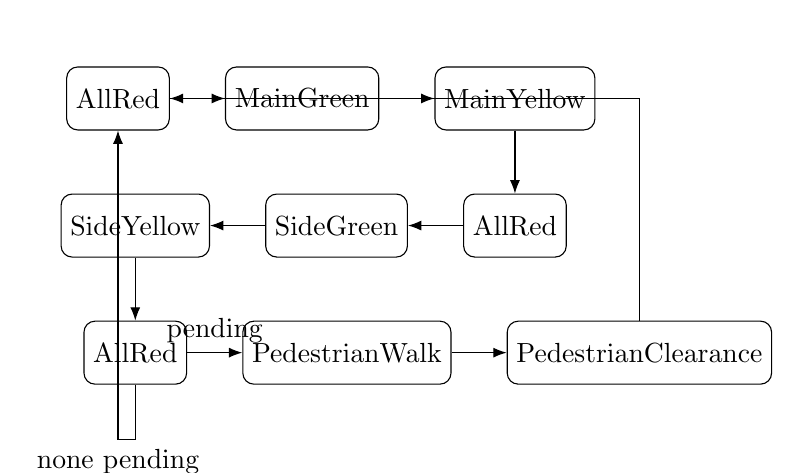
\begin{tikzpicture}[
    node distance=8mm and 7mm,
    phase/.style={draw,rounded corners,minimum height=8mm,align=center},
    >=Latex]
  \node[phase] (all1) {AllRed};
  \node[phase,right=of all1] (mg) {MainGreen};
  \node[phase,right=of mg] (my) {MainYellow};
  \node[phase,below=of my] (all2) {AllRed};
  \node[phase,left=of all2] (sg) {SideGreen};
  \node[phase,left=of sg] (sy) {SideYellow};
  \node[phase,below=of sy] (all3) {AllRed};
  \node[phase,right=of all3] (walk) {PedestrianWalk};
  \node[phase,right=of walk] (clear) {PedestrianClearance};
  \draw[->] (all1) -- (mg);
  \draw[->] (mg) -- (my);
  \draw[->] (my) -- (all2);
  \draw[->] (all2) -- (sg);
  \draw[->] (sg) -- (sy);
  \draw[->] (sy) -- (all3);
  \draw[->] (all3) -- node[above]{pending} (walk);
  \draw[->] (walk) -- (clear);
  \draw[->] (clear) |- (all1);
  \draw[->] (all3.south) -- ++(0,-7mm) -| node[below]{none pending} (all1.south);
\end{tikzpicture}
\end{center}

The first \texttt{update()} anchors startup \texttt{AllRed}; it does not borrow
time from construction or from Arduino's global clock. Every later transition
occurs when the supplied \texttt{TimePoint} reaches the exact deadline. A press
event becomes a pending request. Startup may serve it immediately after
startup all-red; otherwise the controller retains it until the next safe
pedestrian window after the side-road sequence.

\begin{tabularx}{\linewidth}{@{}l X X@{}}
\toprule
Phase & Lamps that are on & Invariant\\
\midrule
AllRed & main red, side red, pedestrian stop & no vehicle green\\
MainGreen & main green, side red, pedestrian stop & one vehicle green\\
MainYellow & main yellow, side red, pedestrian stop & no vehicle green\\
SideGreen & main red, side green, pedestrian stop & one vehicle green\\
SideYellow & main red, side yellow, pedestrian stop & no vehicle green\\
PedestrianWalk & both vehicle reds, pedestrian walk & vehicles held red\\
PedestrianClearance & both vehicle reds, pedestrian stop & vehicles held red\\
Fault & both vehicle reds, pedestrian stop & latched until explicit reset\\
\bottomrule
\end{tabularx}

\section{Orientation drawing}

\begin{figure}[ht]
  \centering
  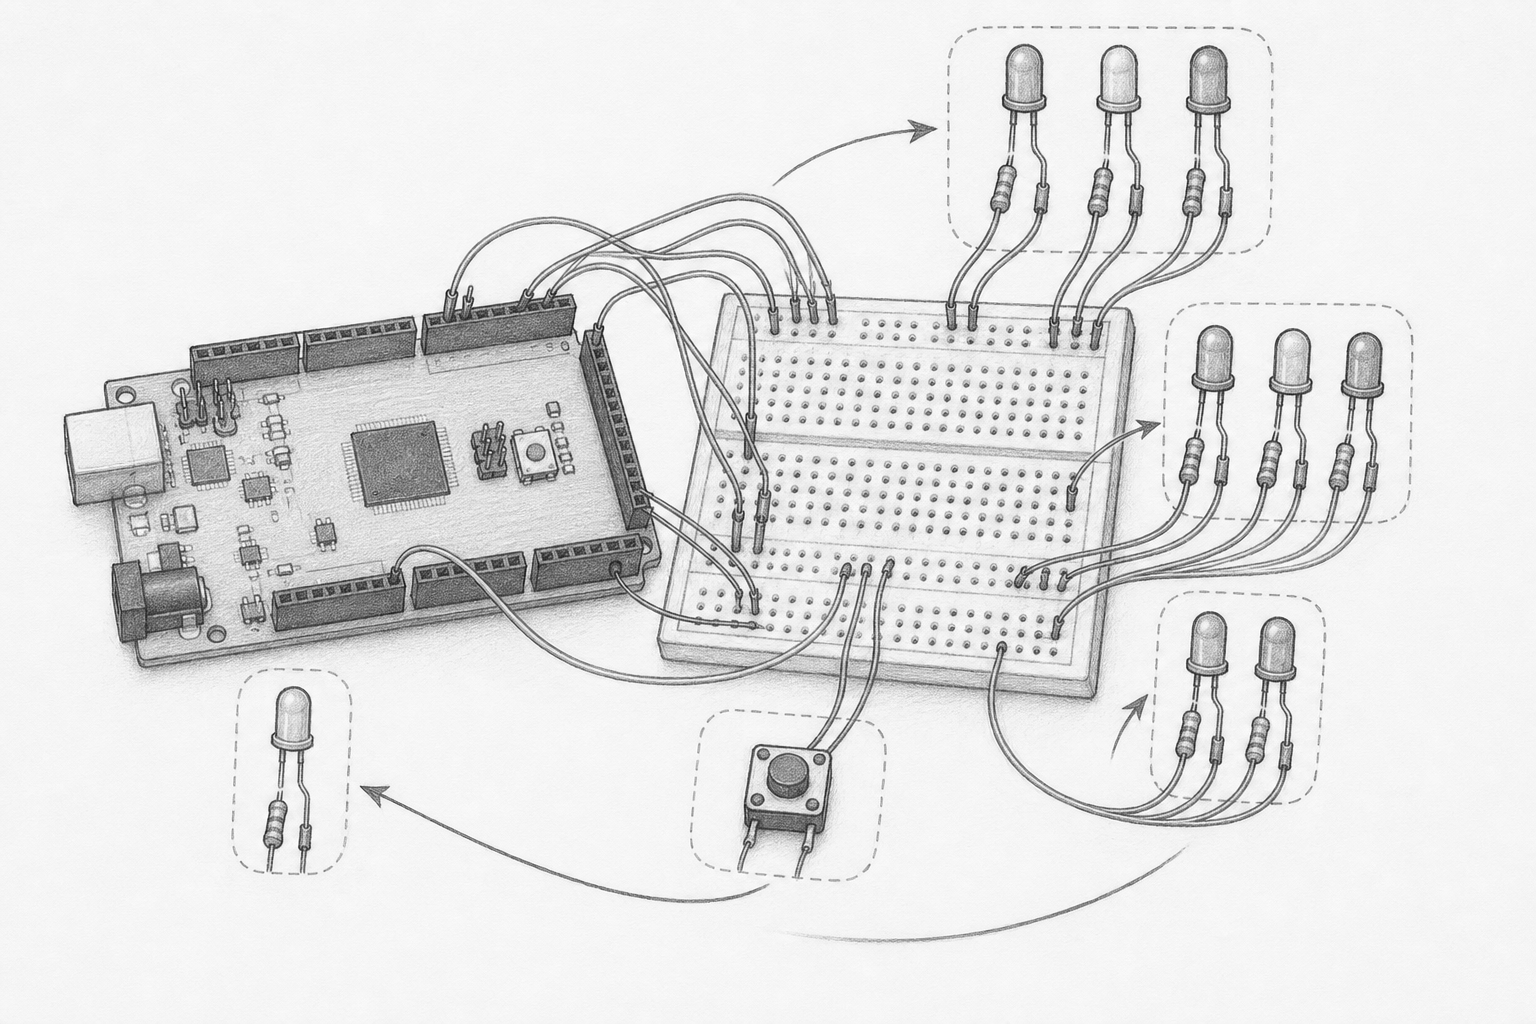
\includegraphics[width=\linewidth]{011-timed-traffic-pencil.png}
  \caption{Pencil orientation showing two vehicle lamp groups, a pedestrian
  lamp pair, request button, ready indicator, Mega, and breadboard. This is not
  an authoritative wiring diagram; build only from the literal connection
  table below.}
\end{figure}

\section{Parts and literal wiring}

\begin{tabularx}{\linewidth}{@{}l l X@{}}
\toprule
Quantity & Part & Requirement\\
\midrule
1 & Mega 2560 & USB powered\\
4 & red LEDs & identified polarity and forward-voltage range\\
2 & yellow LEDs & identified polarity and forward-voltage range\\
3 & green LEDs & two vehicle, one pedestrian/ready as assigned below\\
9 & resistors & 330\(\Omega\) or larger, one per LED\\
1 & momentary button & normally open, used with internal pull-up\\
1 & multimeter & DC voltage and unpowered continuity\\
\bottomrule
\end{tabularx}

\textbf{Every LED path:} named Mega pin \(\rightarrow330\,\Omega\rightarrow\)
LED anode; LED cathode \(\rightarrow\) GND. D22 connects through the normally
open button to GND; \texttt{Pull::Up} supplies its idle level.

\begin{tabularx}{\linewidth}{@{}l l l@{}}
\toprule
Function & Pin & Circuit-native observation\\
\midrule
main red / yellow / green & D30 / D31 / D32 & main signal head\\
side red / yellow / green & D33 / D34 / D35 & side signal head\\
pedestrian walk / stop & D36 / D37 & pedestrian signal head\\
request button & D22 to GND & press event; pending state appears later as walk\\
resource ready & D13 & on only after all objects initialize\\
electrical test point & selected lamp pin to GND & near 0\,V off; near 5\,V on\\
\bottomrule
\end{tabularx}

With a conservative 2.0\,V LED forward voltage, a 330\(\Omega\) resistor
permits about \((5-2)/330=9.1\) mA. The normal truth table lights four LEDs at
most when D13 ready is included. Record actual forward voltages and currents;
do not substitute assumed values for bench evidence.

\section{Read the public model}

\begin{lstlisting}[style=adkcpp]
adk::TrafficConfig config;
adk::TrafficJunction traffic (config);

traffic.initialize ();
traffic.update (now, adk::TrafficInput (requestEvent, circuitHealthy));

const adk::TrafficSnapshot decision = traffic.snapshot ();

traffic.reset    ();
traffic.shutdown ();
\end{lstlisting}

\texttt{TrafficConfig} names each duration:
\texttt{startupAllRed}, \texttt{vehicleAllRed}, \texttt{mainGreen},
\texttt{mainYellow}, \texttt{sideGreen}, \texttt{sideYellow},
\texttt{pedestrianWalk}, and \texttt{pedestrianClearance}. Defaults are
1,000; 500; 5,000; 1,500; 4,000; 1,500; 5,000; and 2,000 ms respectively.

\texttt{TrafficSnapshot} exposes phase and status, output signals, phase start
and next deadline, request state, change and acceptance events, deadline
presence, and transition count:

\begin{lstlisting}[style=adkcpp]
phase, status, signals,
phaseSince, nextDeadline,
pedestrianRequestPending,
phaseChanged, requestAccepted, hasDeadline,
transitionCount
\end{lstlisting}

Observation does not consume an event. Supplying the same configuration,
timestamps, and input events produces the same snapshots. Repeated
\texttt{initialize()} is idempotent: it preserves the active phase, timing,
pending request, or fault latch. \texttt{reset()} explicitly starts a new run
in startup \texttt{AllRed}; it requires an initialized object.
\texttt{shutdown()} is idempotent, leaves an inert all-red snapshot, and makes
later \texttt{update()} calls report \texttt{NotInitialized}.

The canonical sketch uses the same high-level language as the circuit:

\begin{lstlisting}[style=adkcpp]
const adk::TrafficInput observation = observeRequest (now);
const adk::Status       decision    = decideSignals  (now, observation);
const bool              signalsShown = showSignals   (traffic.snapshot ().signals);

if (!signalsShown)
{
    stopSafely ();
}

if (decision != adk::Status::Ok)
{
    ready.off ();
}
\end{lstlisting}

There is no \texttt{delay()}. \texttt{loop()} remains free to debounce the
button and actuate the current signal during every phase. The complete,
canonical source is
\href{https://github.com/spincyc/adk/tree/main/examples/Lesson011TimedTraffic}
{Lesson011TimedTraffic}.

\section{CLI experiment}

\begin{enumerate}
  \item With USB disconnected, check every LED path and confirm no short from
        5\,V to GND.
  \item Predict the startup lamps and the first four deadlines.
  \item Build with \texttt{make arduino-Lesson011TimedTraffic}.
  \item Upload with
        \texttt{make upload-Lesson011TimedTraffic PORT=/dev/ttyACM0}.
  \item Observe D13 ready separately from the eight policy lamps.
  \item Press D22 briefly during \texttt{MainGreen}. Continue watching: the
        request is retained, not served by interrupting a vehicle phase.
  \item Measure D32 to GND during main green and all-red; record both voltages.
  \item Optional supporting evidence:
        \texttt{make serial-log PORT=/dev/ttyACM0}. The sketch needs no Serial
        log to prove its state.
\end{enumerate}

\evidencebox{\textbf{Predict.} A request during main green cannot immediately
turn on walk. \textbf{Observe.} Main completes, side completes, both vehicle
reds appear, then walk appears. \textbf{Interpret.} The event was latched and
served only at a designed boundary. This evidence does not by itself prove the
pin voltages or resource cleanup.}

\section{Deterministic trace worksheet}

Use shortened test durations on the host, not on an unexplained bench circuit:
startup all-red 100 ms, vehicle all-red 50 ms, main green 300 ms, main yellow
100 ms, side green 200 ms, side yellow 100 ms, walk 250 ms, clearance 150 ms.

\begin{tabularx}{\linewidth}{@{}r l l X@{}}
\toprule
Time & Input event & Predicted phase & Snapshot evidence\\
\midrule
0 ms & none & \blank{2.7cm} & deadline \blank{2.5cm}\\
100 ms & none & \blank{2.7cm} & transition count \blank{1.5cm}\\
220 ms & request & \blank{2.7cm} & pending \blank{1.5cm}\\
400 ms & none & \blank{2.7cm} & lamps \blank{3.0cm}\\
500 ms & none & \blank{2.7cm} & deadline \blank{2.5cm}\\
700 ms & none & \blank{2.7cm} & lamps \blank{3.0cm}\\
800 ms & none & \blank{2.7cm} & pending \blank{1.5cm}\\
850 ms & none & \blank{2.7cm} & lamps \blank{3.0cm}\\
\bottomrule
\end{tabularx}

Replay the table twice. Compare every snapshot field, not merely the final
phase. Then shift the request to the startup all-red interval and explain why
the service order changes without becoming nondeterministic.

\section{Faults, diagnosis, and safe evidence}

Passing \texttt{TrafficInput(false, false)} enters \texttt{Fault}, selects both
vehicle reds and pedestrian stop, returns a failure status, and latches that
condition. Repeated \texttt{initialize()} deliberately preserves this latch;
only \texttt{reset()} begins a new run. The adapter presents the all-red fault
signals and turns D13 off. It treats an output-write failure more
conservatively: it shuts down the state engine and every \texttt{MonoLed},
making each owned output high impedance.

\begin{tabularx}{\linewidth}{@{}l X X@{}}
\toprule
Observation & Likely layer & Next evidence\\
\midrule
D13 never lights & acquisition or wiring & unpowered continuity; inspect pin claims\\
D13 lights, one head dark & LED path or actuation & measure the named pin and resistor\\
request never served & input wiring or event timing & observe D22 and button debounce\\
walk interrupts green & policy defect & stop; preserve timestamp/input trace\\
both greens appear & invariant violation or wiring & remove USB immediately\\
lamps freeze but loop runs & timestamp/configuration & inspect deadlines with host trace\\
all lamps extinguish after failure & application safe shutdown & measure high impedance\\
\bottomrule
\end{tabularx}

\textbf{Resource evidence} is D13 turning on only after ten pin owners and the
state engine initialize. \textbf{Policy evidence} is the truth-table lamp
pattern. \textbf{Safe-state evidence} after an application failure is the
measured high-impedance output, not merely a dark LED. These are three separate
claims.

\section{Exercises}

\begin{enumerate}
  \item Draw the exact phase reached at every default deadline for one complete
        cycle with no request.
  \item Record two request events during one cycle. Explain why one pending bit
        is sufficient for this lesson and what information it intentionally
        does not count.
  \item Add a circuit-native pending indicator in a host-only design. State its
        extra pin and current cost before changing hardware.
  \item Inject decreasing time, a zero duration, and an unhealthy circuit into
        deterministic tests. Predict the returned \texttt{Status}.
  \item Explain why a blinking pedestrian-clearance display belongs in a
        presentation adapter rather than hidden timing inside the engine.
  \item Propose a power-on lamp test that does not weaken the all-red invariant.
\end{enumerate}

\section{Bench acceptance record}

Do not mark this lesson hardware verified until every blank is measured.

\begin{tabularx}{\linewidth}{@{}l X@{}}
\toprule
Record & Observation\\
\midrule
Board and supply & Mega 2560 revision \blank{2cm}; USB supply \blank{2cm}\\
Resistors & D13, D30--D37 measured values \blank{7cm}\\
Startup & D13 sequence \blank{2cm}; initial signal pattern \blank{3cm}\\
Normal cycle & observed phase order and durations \blank{6cm}\\
Request & press phase \blank{2cm}; served phase/time \blank{3cm}\\
Electrical & D32 on \blank{1.5cm} V; off \blank{1.5cm} V; reference GND \blank{2cm}\\
Reset & observed startup all-red behavior \blank{5cm}\\
Shutdown & selected output high-impedance measurement \blank{4cm}\\
Current & maximum simultaneous LED current \blank{2cm} mA\\
Tools & meter/model \blank{3cm}; CLI/core versions \blank{3cm}\\
Result & \checkbox\ pass \quad \checkbox\ deviation attached \quad date/reviewer \blank{3cm}\\
\bottomrule
\end{tabularx}

\textbf{Current status: host verified and Mega 2560 firmware compiled; physical
bench acceptance remains open until the completed record is published.}

\end{document}
